\section{Background}
\label{sec:background}

Arguing about the security of an application running on an mainstream computer
using the Intel architecture requires understanding the interactions between
all the parts of an x86 execution environment. This section provides an
overview of the features referenced by the rest of the paper. The section is
written from the context of SGX, but does not introduce any SGX concepts, so
most experienced readers can safely skip the section and refer back if
necessary.


\subsection{Software Privilege Levels}
\label{sec:rings}

In an Infrastructure-as-a-Service (IaaS) cloud environment, such as Amazon EC2,
commodity CPUs run software at four different privilege levels, illustrated in
Figure~\ref{fig:cpu_rings} and described below. The rest of the section
describes the privilege levels. We also point to successful exploits that
execute at each privilege level, motivating the SGX design decision to assume
that the host computer has malicious software running at all privilege levels.

\begin{figure}[hbtp]
  \center{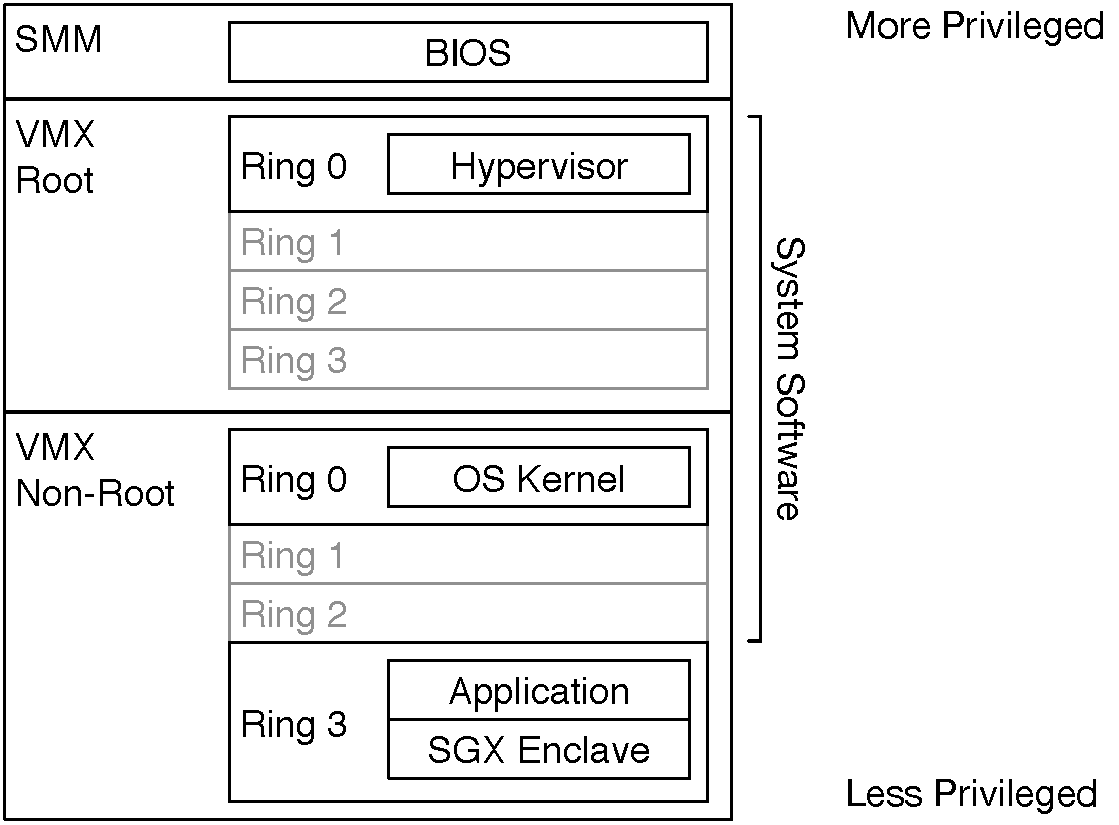
\includegraphics[width=50mm]{figures/cpu_rings.pdf}}
  \caption{
    The privilege levels in the x86 architecture, and the software that
    typically runs at each security level.
  }
  \label{fig:cpu_rings}
\end{figure}

\textit{System Management Mode} (SMM) is intended for use by the motherboard
manufacturers to implement features such as fan control and deep sleep, and/or
to emulate missing hardware. SMM mode is entered by asserting the SMI\# pin on
the CPU, which was initially designed exclusively for hardware use. However,
the southbridges on most motherboards provide a method for privileged
code\footnote{the hypervisor or operating system kernel} to get the SMI\# pin
asserted\footnote{Most southbridges assert \texttt{SMI\#} when a byte is
  written to port 0xb2 via the \textsc{out} opcode}.
This opens up the avenue for SMM-based software exploits.

The SMM code and data are stored in a contiguous subset of RAM called
\textit{System Management RAM} (SMRAM), which, in theory, is not readable or
writable when the processor isn't running in SMM. However, its protection
mechanisms were bypassed multiple times \cite{duflot2006smm}
\cite{rutkowska2008remap} \cite{wojtczuk2009smm}, and SMM-based rootkits have
been demonstrated \cite{wecherowski2009smm} \cite{embleton2010smm}.

IaaS cloud providers allow their customers to run their operating system of
choice in a virtualized environment. Hardware
virtualization\cite{uhlig2005vmx}, called \textit{Virtual Machine Extensions}
(VMX) by Intel, adds support for a \textit{hypervisor}, also called a
Virtual Machine Monitor (VMM) in the Intel documentation. The hypervisor runs
at a higher privilege level (VMX root mode) than the operating system, and is
responsible for allocating hardware resources across multiple operating systems
that share the same physical machine. The hypervisor uses the CPU's hardware
virtualization features to make each operating system believe it is running in
its own computer, called a \textit{virtual machine} (VM). Hypervisor code
generally runs at ring 0 in VMX root mode.

The popular Xen hypervisor uses VMX root mode for improved peformance and a
smaller codebase \cite{zhang2008xen}. \cite{mccune2010trustvisor} proposes
using a hypervisor together with Intel TXT's dynamic root of trust for
measurement (DRTM) to implement trusted execution.
\cite{vasudevan2010requirements} argues that a dynamic root of trust mechanism,
like Intel TXT, is necessary to ensure a hypervisor's integrity. Unfortunately,
the TXT design requires an implementation complex enough that security
vulnerabilities have been found \cite{wojtczuk2009txt2} \cite{wojtczuk2011txt}.
Furthermore, any SMM attack can be used to compromise TXT
\cite{wojtczuk2009txt}.

The systems research literature recommends breaking up an operating system into
a small \textit{kernel}, which runs at a high privilege level, known as the
\textit{kernel mode} or \textit{system mode} and, in the Intel architecture, as
\textit{ring 0}. The kernel allocates the computer's resources to the other
system components, such as device drivers and services, which run at lower
privilege levels. However, for performance reasons\footnote{Switching between
rings is much slower than a normal procedure call.}, mainstream operating
systems have large amounts of code running at ring 0. Their \textit{monolithic
kernels} include device drivers, filesystem code, networking stacks, and video
rendering functionality.

The monolithic kernel design leads to many opportunities for security
vulnerabilities in kernel code. For example the Linux kernel has had a
significant number of vulnerabilities patched every year, for the past 10 years
\cite{cvedetails2014linux} \cite{chen2011linux}. Also, a successful attack on
SMM or the hypervisor trivially translates into a compromised kernel.

Application code, such as a Web server or a game client, runs at the lowest
privilege level, referred to as \textit{user mode} (\textit{ring 3} in the
Intel architecture). In IaaS cloud environments, the virtual machine images
provided by customers run in VMX non-root mode, so the kernel runs in VMX
non-root ring 0, and the application code runs in VMX non-root ring 3.


\subsection{Address Translation}
\label{sec:paging}

The software running inside an enclave is subject to address translation, which
is used by the hypervisor and kernel to multiplex a computer's memory across
virtual machines and applications. This section summarizes the address
translation details specific to the Intel architecture. \cite{jacob1998virtual}
describes the generic concepts and applications of address translation.

The Intel architecture specifies many address translation modes, used to run
legacy software dating back to 1990 natively. Most modes are not necessary for
understanding SGX, so we only cover the translation modes used in modern 64-bit
operating systems and 64-bit cloud environments.

64-bit desktop operating systems use the addressing mode called IA-32e in
Intel programming manual \cite{intel2013manual}, which translates 48-bit
\textit{virtual addresses} into \textit{physical addresses} of at most 52
bits\footnote{The size of a physical address is CPU-dependent, and is 40 bits
for recent desktop CPUs and 44 bits for recent high-end server CPUs.}.
Figure~\ref{fig:os_paging} illustrates the address translation process. The
bottom 12 bits of a virtual address are not changed by the translation. The top
36 bits are grouped into four 9-bit indexes used to navigate a data structure
called \textit{the page tables}. Despite its name, the data structure closely
resembles a perfectly balanced 512-ary search tree where the nodes do not store
keys. Each node is an array of 512 8-byte entries that contain the physical
addresses of the next-level children as well as some flags. The address of the
root node is stored in the CR3 register. The arrays in the last-level nodes
contain the physical addresses that are the result of the address translation.

\begin{figure}[hbtp]
  \center{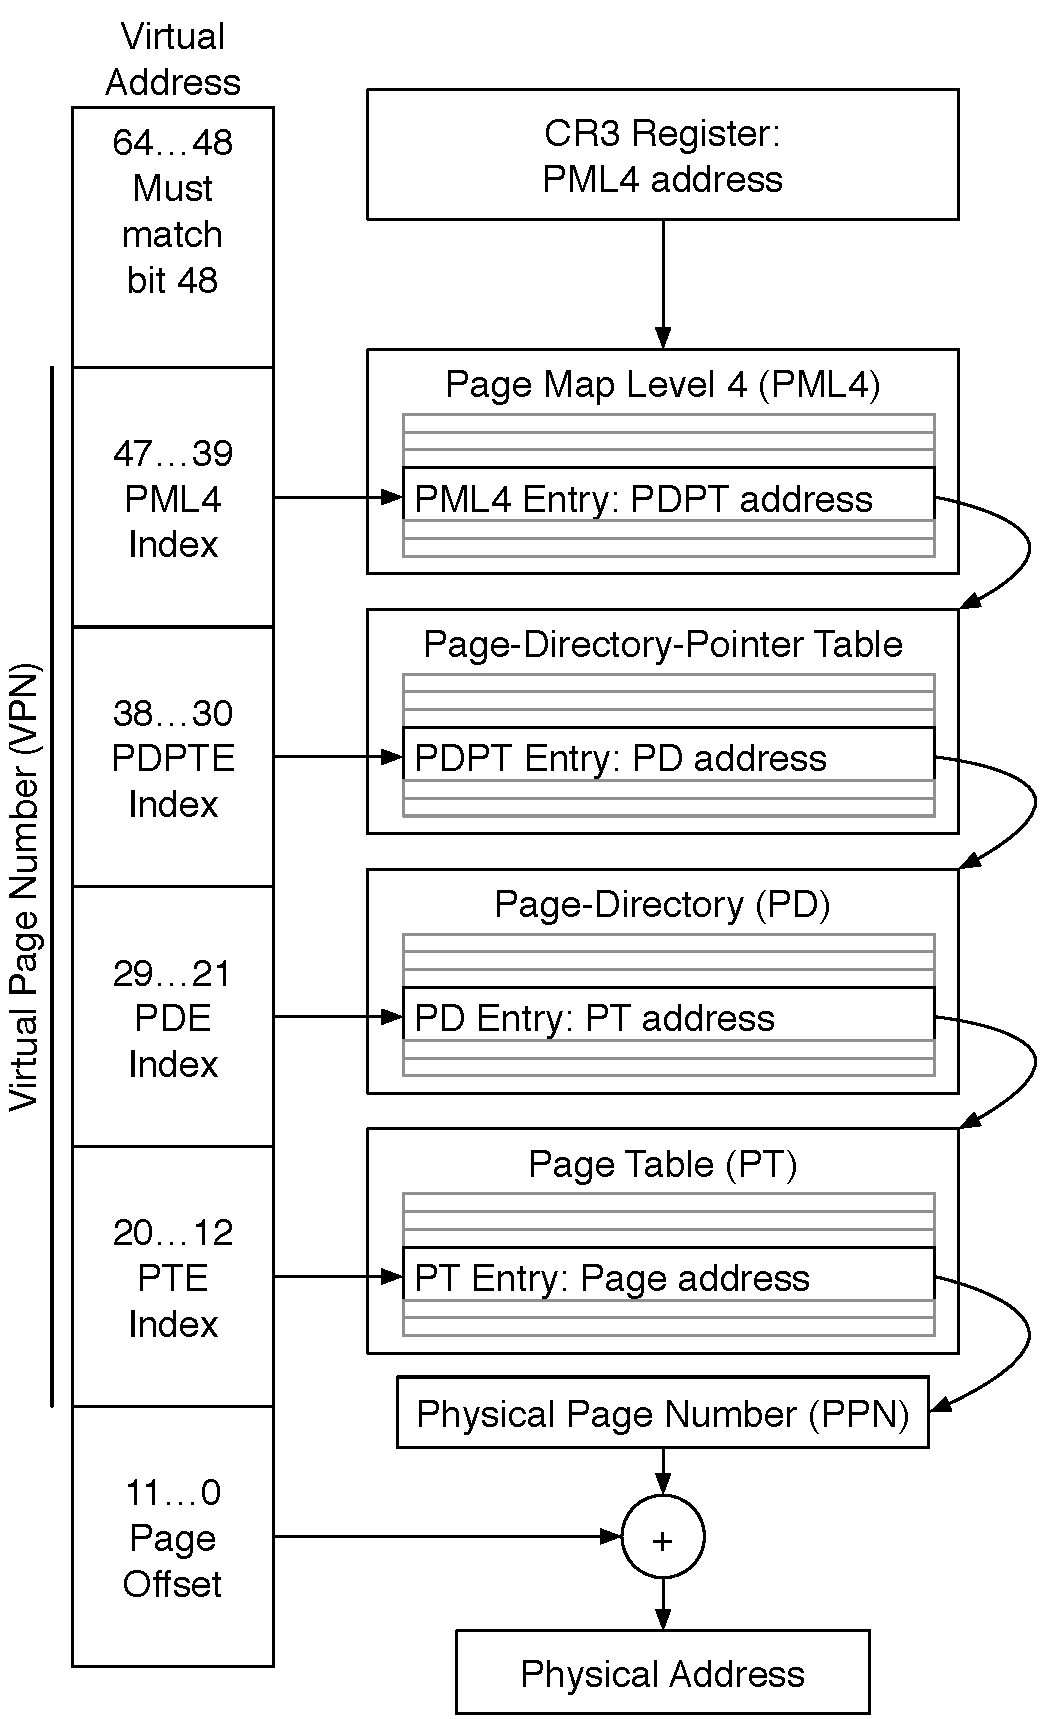
\includegraphics[width=85mm]{figures/os_paging.pdf}}
  \caption{
    IA-32e address translation takes in a 48-bit virtual address and outputs
    a 52-bit physical address.
  }
  \label{fig:os_paging}
\end{figure}

Hardware virtualization (used in cloud computing) allows a hypervisor to run
multiple operating systems concurrently using the same physical memory, by
adding another layer of address translation, named the \textit{extended page
tables} (EPT). When EPT are enabled, the process above is used to translate
from a virtual address into a \textit{guest-physical address}. The translation
from guest-physical addresses to actual physical addresses uses the same
process as above, except the physical address of the root node is stored in the
extended page table pointer (EPTP) field in the VM's control structure (VMCS).
Figure~\ref{fig:vmx_paging} illustrates the address translation process in the
presence of hardware virtualization.

\begin{figure}[hbtp]
  \center{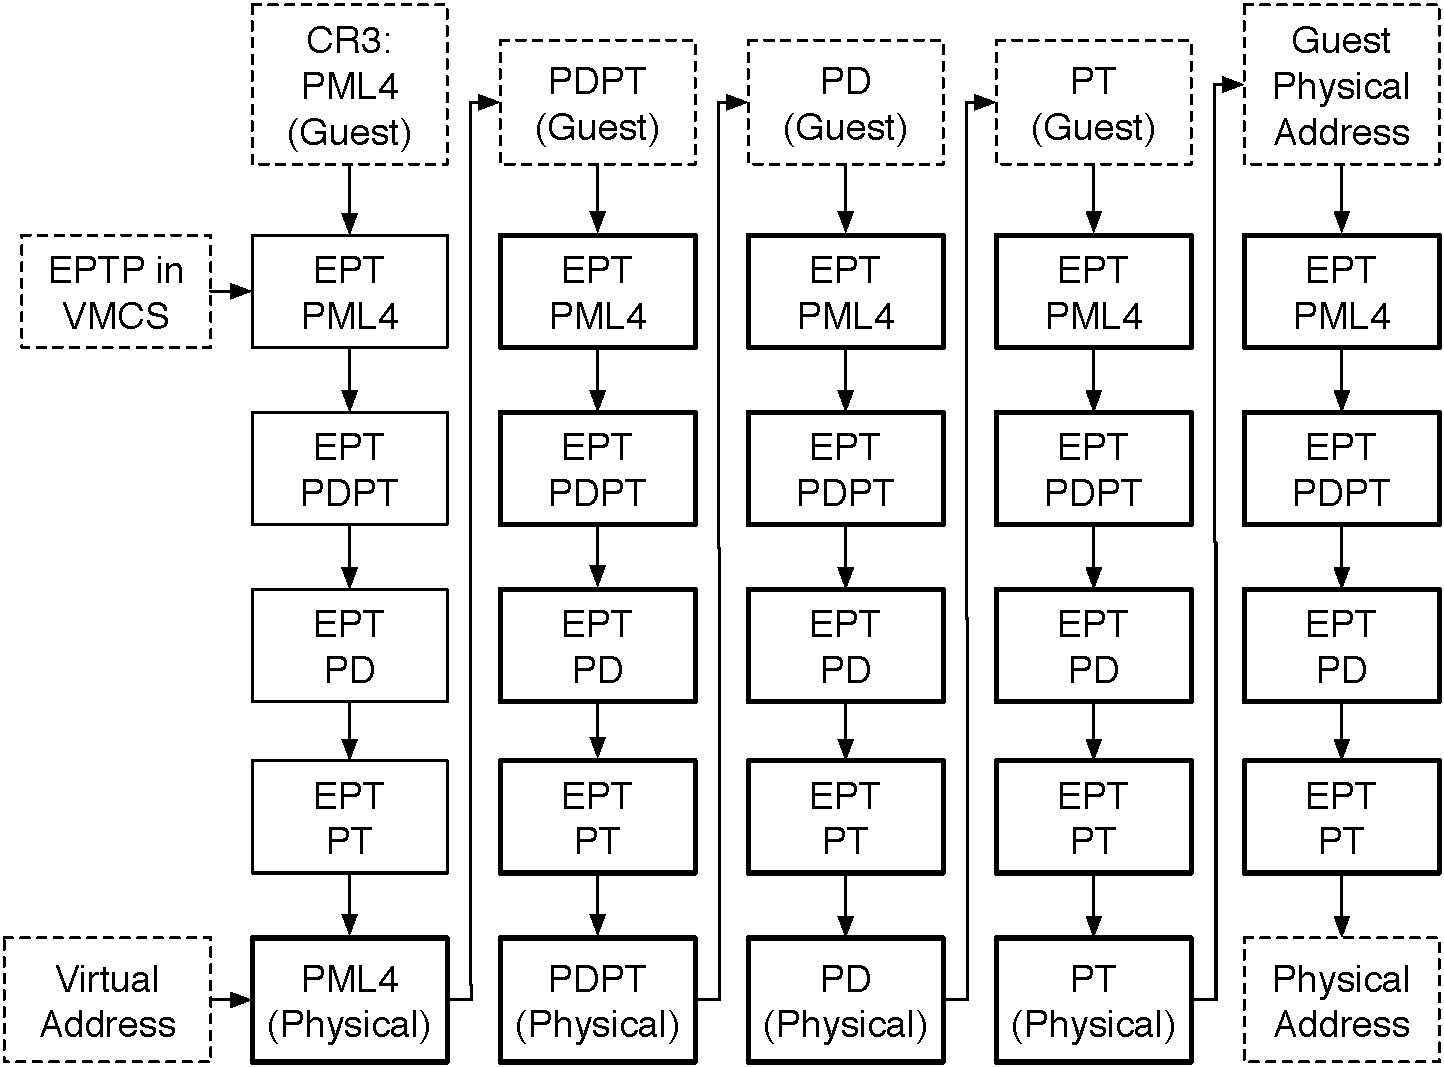
\includegraphics[width=85mm]{figures/vmx_paging.pdf}}
  \caption{
    Address translation when hardware virtualization is enabled. A translation
    requires up to 16 memory accesses.
  }
  \label{fig:vmx_paging}
\end{figure}

Each entry in the page tables has some boolean flags, in addition to the
pointer to the next level. The following flags are particularly interesting for
our goals. The \textit{present} (P) flag is set to 0 to indicate pages that
have been evicted from RAM to a cheaper and slower storage medium. When address
translation encounters a page table entry where P is 0, the CPU generates a
page fault (\#PF), and the OS kernel is responsible for loading the page back
into RAM and resuming execution. If an EPT entry has the P flag set to 0, the
CPU performs a VM exit, and the hypervisor has an opportunity to bring the page
into RAM. The \textit{accessed} (A) flag is set to 1 by the CPU whenever the
address translation machinery reads a page table entry, and the \textit{dirty}
(D) flag is set to 1 by the CPU when an entry is accessed by a memory write
operation. The A and D flags give the hypervisor and kernel insight into
application memory access patterns, providing the input for the algorithms that
select which pages get to be evicted from RAM.

Page table entries have flags that provide access control, in addition to the
flags supporting page swapping. The interesting flags are the \textit{writable}
(W) flag, which can be set to 0 to prohibit\footnote{Writes to non-writable
pages result in general protection faults (\#GP).} memory writes to a page, and
the \textit{disable execution} (XD) flag, which can be set to 0 to prevent
instruction fetches from a page.


\subsection{Logical Processors}
\label{sec:cores}

Modern CPUs have multiple execution cores, and each core independently executes
a stream of instructions (\textit{hardware thread} in the Intel documentation).
The cores are exposed to system software as \textit{logical processors}, so
that the code used to distribute work across processors in a multi-processor
system works without changes on multi-core processors. This section covers the
details in Intel's multi-core implementation needed to understand the aspects
of SGX that support having multiple hardware threads running code in the same
enclave, as well as the security implications of this design decision.

\begin{figure}[hbt]
  \center{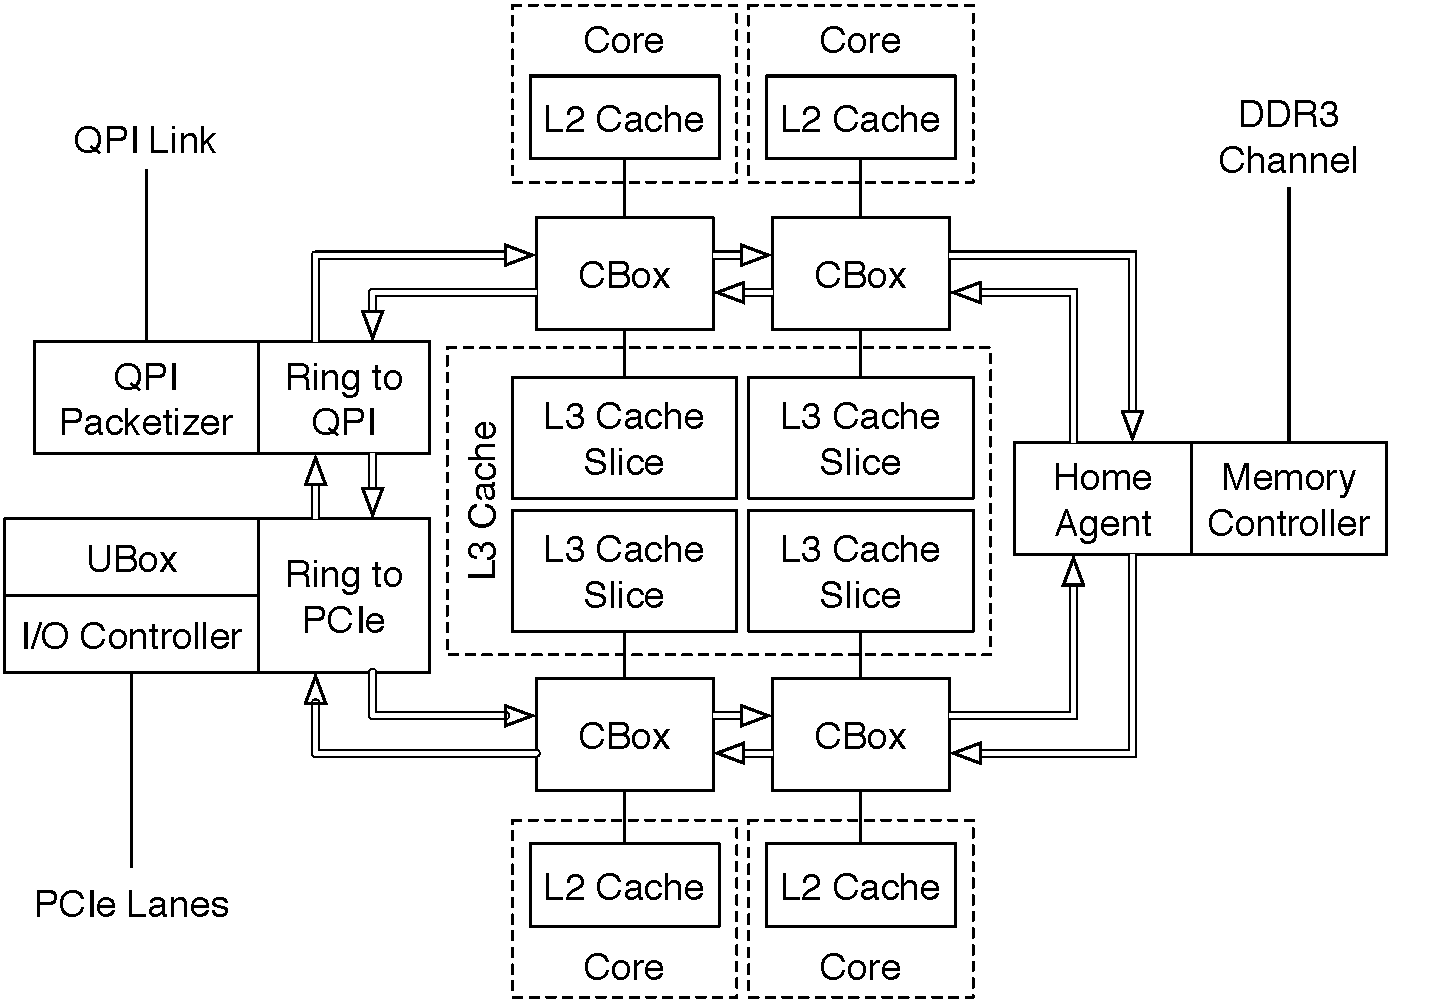
\includegraphics[width=85mm]{figures/cpu_die.pdf}}
  \caption{
    A modern CPU die contains multiple cores. The cores share some on-chip
    resources, such as the L3 cache and the memory controller.
  }
  \label{fig:cpu_die}
\end{figure}

At the time of this writing, desktop-class Intel CPUs have 4 cores, and
server-class CPUs have as many as 18 cores. The cores share the L3 cache
(described in \S~\ref{sec:caching} below) and other on-chip resources, such as
the memory controller, and controllers that interface with the system buses
(see Figure~\ref{fig:cpu_die}).

\begin{figure}[hbt]
  \center{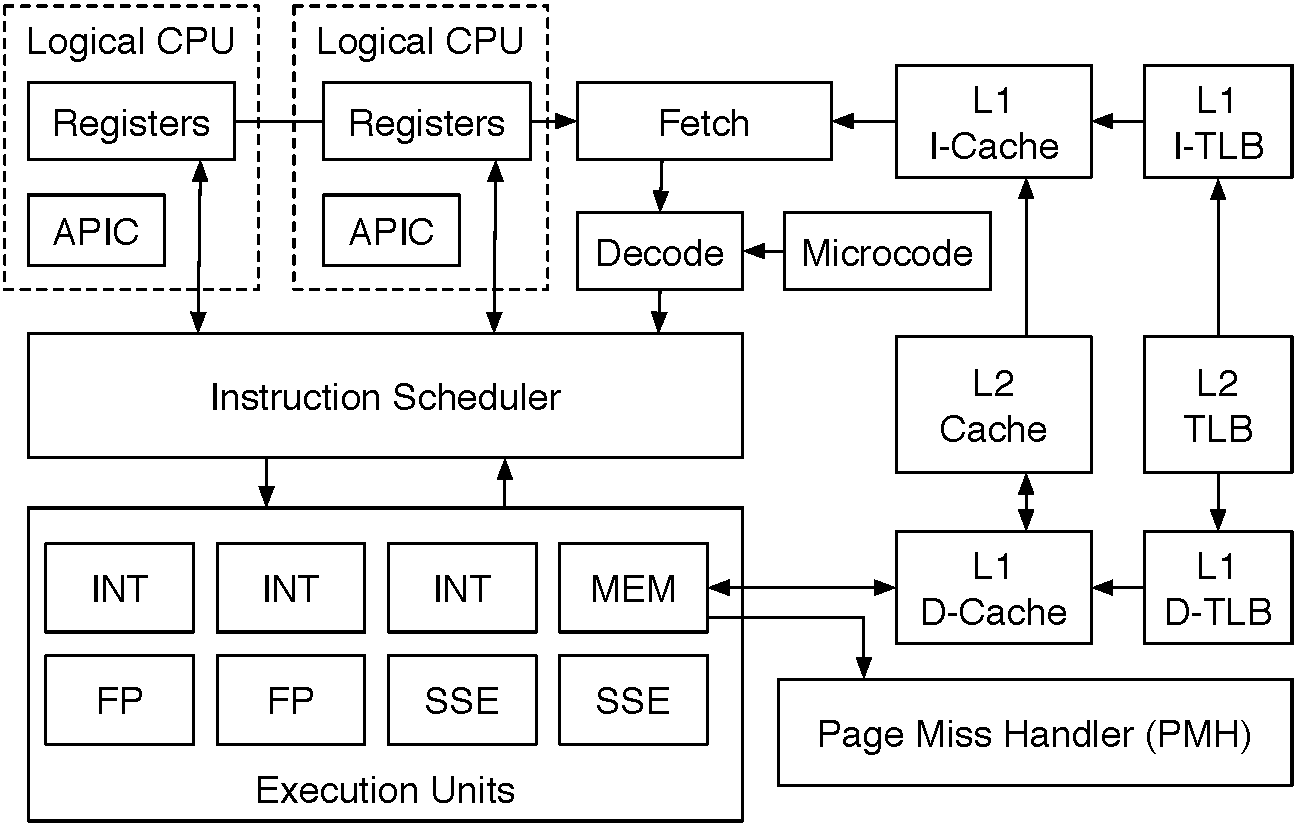
\includegraphics[width=85mm]{figures/cpu_core.pdf}}
  \caption{
    CPU core with two logical processors. Each logical processor has its own
    APIC and execution state, and they share all the other core resources.
  }
  \label{fig:cpu_core}
\end{figure}

Most Intel CPUs also feature \textit{hyper-threading}, which means that each
core has two (or more) sets of register files and local APICs (see
Figure~\ref{fig:cpu_core}), exposed as separate logical processors. The
logical processors share many core resources, such as the fetch and decode
units, the execution units, and the L1 and L2 caches (described in
\S~\ref{sec:caching} below). This has security implications, as software
running on one logical processor can use the high-performance counter
\cite{petters1999making} to get information about the instructions and memory
access patterns of another piece of software that is executed on another
logical processor in the same core.


\subsection{CPU Caches}
\label{sec:caching}

Caches are small, fast memories that store recently accessed code and data.
Thanks to the high locality in the memory access patterns of most applications,
good caches have very high hit rates (90\%-99\%), and do a great job of hiding
the (comparatively) high latency of RAM. At the same time, the large time
differences between cached and un-cached memory accesses can be used to learn
about an application's memory access patterns, via
\textit{cache timing attacks}\cite{banescu2011cache}. The patterns, in turn,
can reveal private information, such as whether certain bits in an encryption
key are set or not.

This section describes the caching concepts needed to understand our claim that
cache timing attacks can be used to obtain fine-grained memory access patterns
for the software running inside an SGX enclave. \cite{smith1982cache},
\cite{patterson2013architecture} and \cite{hennessy2012architecture} all
provide good backgrounds on low-level cache implementation concepts.

Desktop-class Intel CPUs have three levels of cache memory. Each core has its
own L1 and L2, and all cores share an L3 cache. This means that a cache timing
attack that aims at the L2 cache would have to rely on the hypervisor or kernel
to schedule a hardware thread on a logical processor in the same core as the
target software, whereas an attack on the L3 cache can be performed using any
logical processor on the same CPU.

The \textit{cache line} is the atomic unit of data transfer between the caches
and the main memory. The cache line size is always a power of two. Assuming
$n$-bit memory addresses and a cache line size of $2^{l}$ bytes, the lowest
$l$ bits of a memory address are an offset into a cache line, and the highest
$n - l$ bits determine the cache line that is used to store the data at the
memory location. All recent processors have 64-byte cache lines.

The L1 and L2 caches in recent processors are multi-way set-associative with
direct set indexing, as shown in Figure~\ref{fig:cpu_cache}. A $W$-way
set-associative cache has its memory divided into \textit{sets}, where each set
has $W$ lines. A memory location can be cached in any of the $w$ lines in a
specific set that is determined by the highest $n - l$ bits of the location's
memory address. Direct set indexing means that the $S$ sets in a cache are
indexed from $0$ to $S - 1$, and a memory location is cached in the set with
index $address_{n - 1 \ldots n - l} \bmod S$. In the common case where the
number of sets in a cache is a power of two, so $S = 2^{s}$, the lowest $l$
bits in an address make up the cache line offset, the next $s$ bits are the set
index. The highest $n - s - l$ bits in an address are not used when selecting
where a memory location will be cached. Figure~\ref{fig:cpu_cache} shows the
cache structure and lookup process.

\begin{figure}[hbt]
  \center{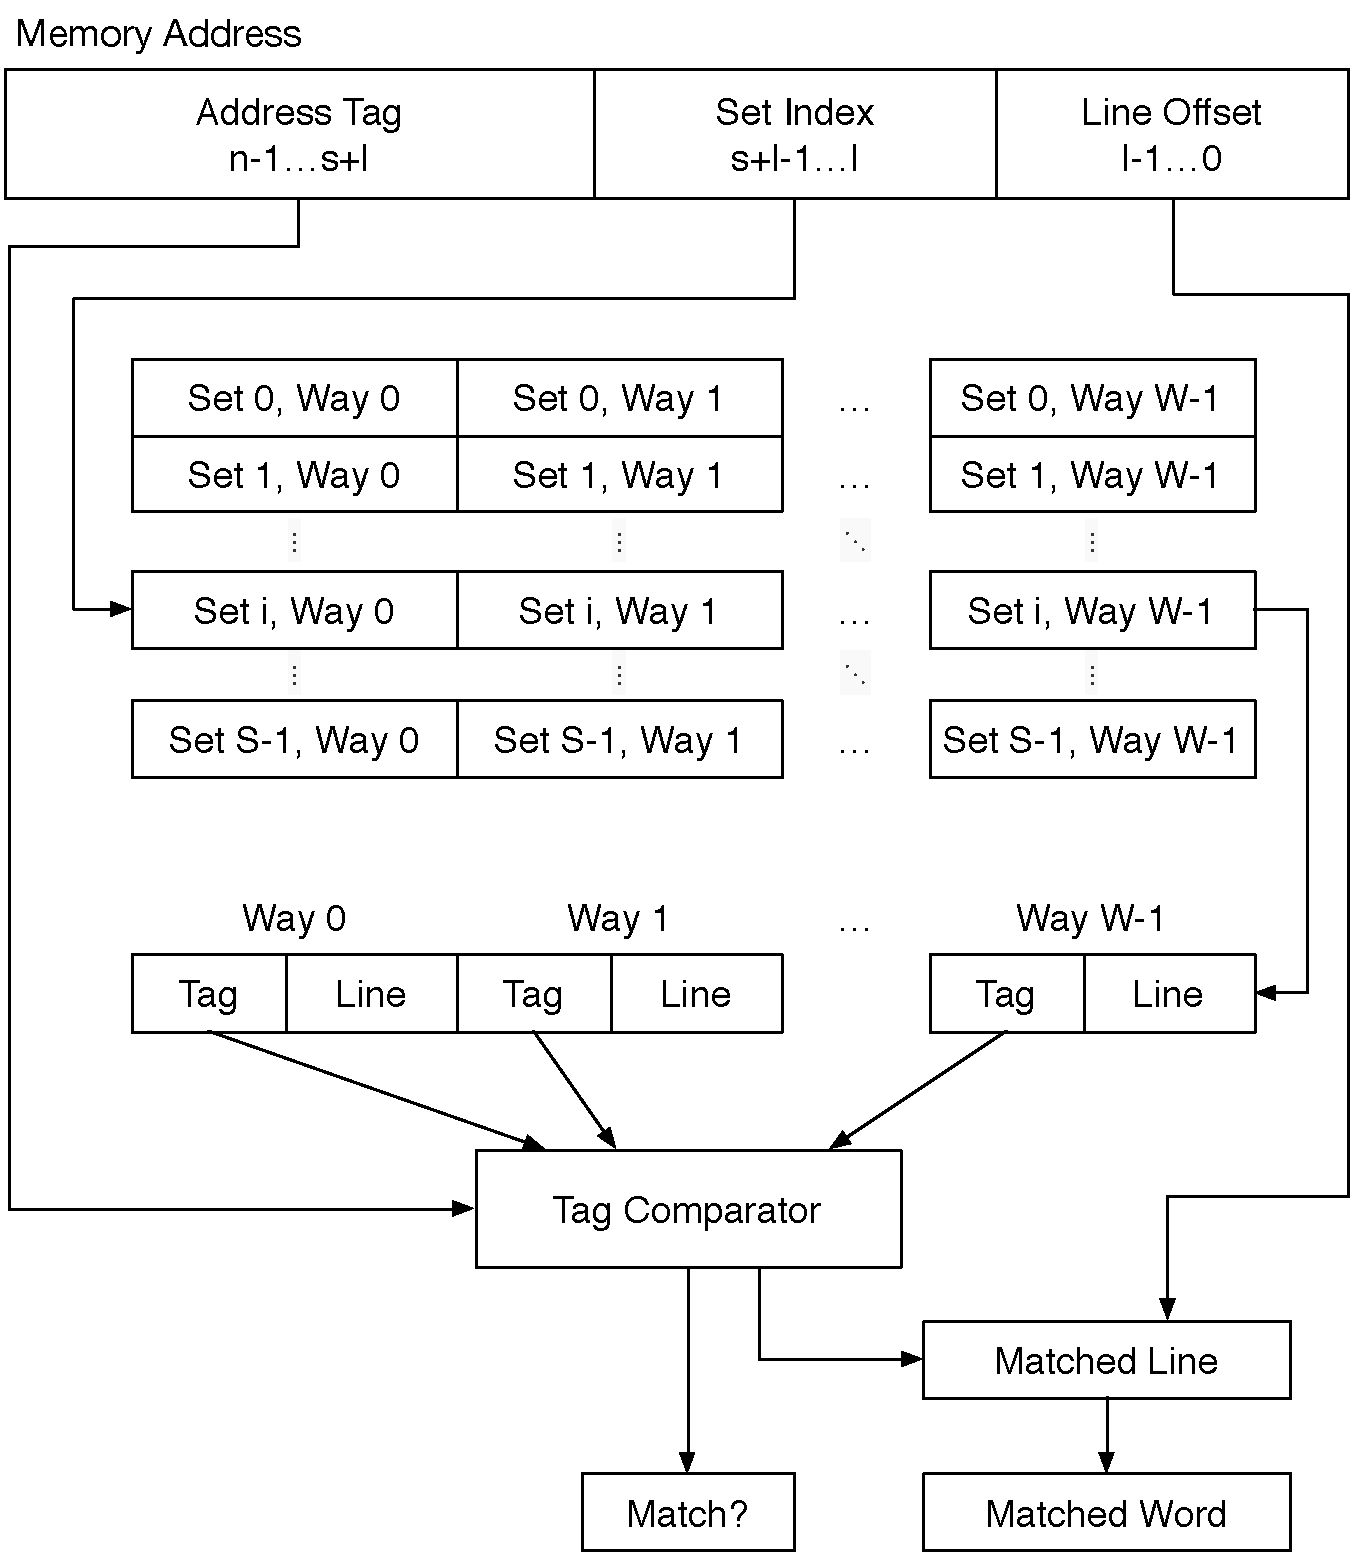
\includegraphics[width=85mm]{figures/cpu_cache.pdf}}
  \caption{
    Cache organization and lookup, for a $W$-way set-associative cache with
    $2^{l}$-byte lines and $S = 2^{s}$ sets. The cache works with $n$-bit
    memory addresses. The lowest $l$ address bits point to a specific byte in a
    cache line, the next $s$ bytes index the set, and the highest $n - s - l$
    bits are used to decide if the desired address is in one of the $W$ lines
    in the indexed set.
  }
  \label{fig:cpu_cache}
\end{figure}

According to the CPUID instruction results and the Intel programming manuals
\cite{intel2013manual}, the L3 cache of recent processors does not use direct
set indexing, and instead uses a ``complex'' indexing scheme, which is not
described in Intel's documentation.


\subsection{Caching and Address Translation}

Address translation (described in \S~\ref{sec:paging}) requires up to 4 memory
accesses for a 64-bit bare-metal kernel, and up to 16 memory accesses when a
hypervisor is present. To achieve high clock speeds, the CPU caches address
translations in a TLB (translation look-aside buffer). The set index in an L1
cache only uses the address bits that are not impacted by address translation,
so that set lookup and TLB lookup can be done in parallel. Given a page size
$P = 2^{p}$ bytes, the requirement above is equivalent to $l + s \le p$. In the
x86 architecture $p = 12$, and all recent processors have 64-byte cache lines
($l = 6$) and 64 sets ($s = 6$), as shown in
Figure~\ref{fig:caching_and_paging}.

\begin{figure}[hbt]
  \center{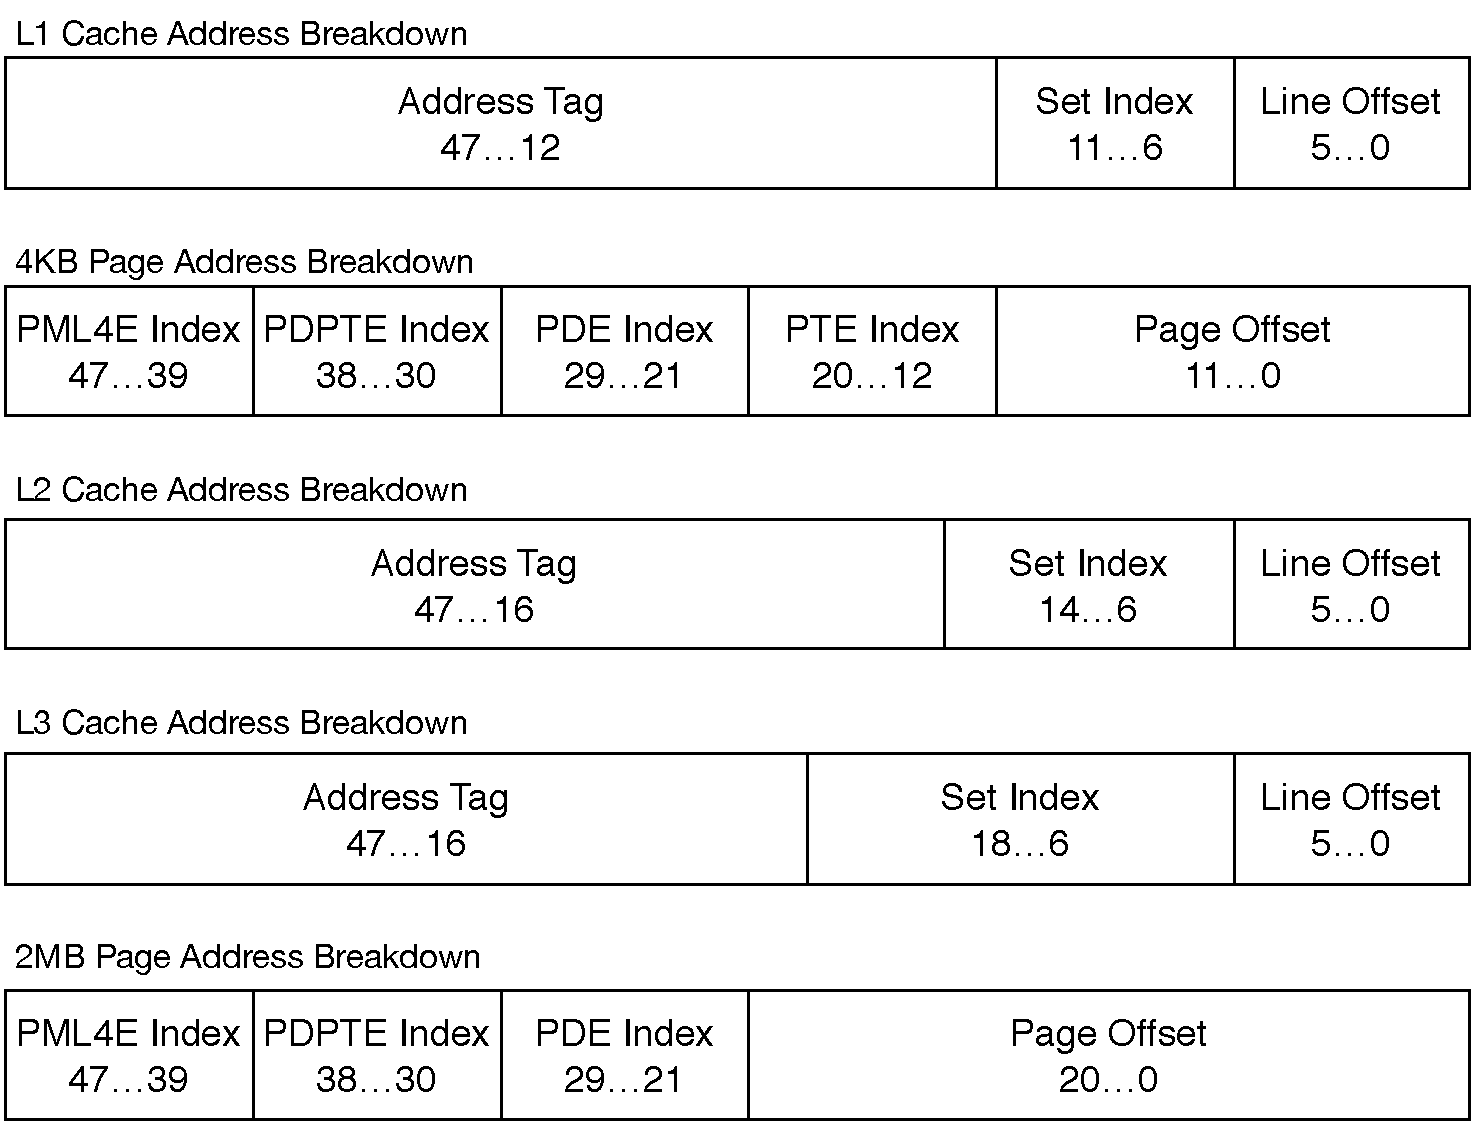
\includegraphics[width=85mm]{figures/caching_and_paging.pdf}}
  \caption{
    Virtual addresses from the perspective of cache lookup and address
    translation. The bits used for the L1 set index and line offset are not
    changed by address translation, so the page tables do not impact L1 cache
    placement. Page tables do impact L2 and L3 cache placement. Using large
    pages (2MB or 1GB) makes cache placement independent of page tables.
  }
  \label{fig:caching_and_paging}
\end{figure}

The L2 cache in recent Intel processors uses physical indexing
\cite{patterson2013architecture}. The indexing method is not documented in
Intel's manuals and is not reported by the CPUID instruction, as it is
considered to be an implementation detail. However, the indexing method
determines the set index for a given memory location, and knowing which memory
addresses are stored in the same set is crucial for mounting and defending
against cache timing attacks.

\begin{figure}[hbt]
  \center{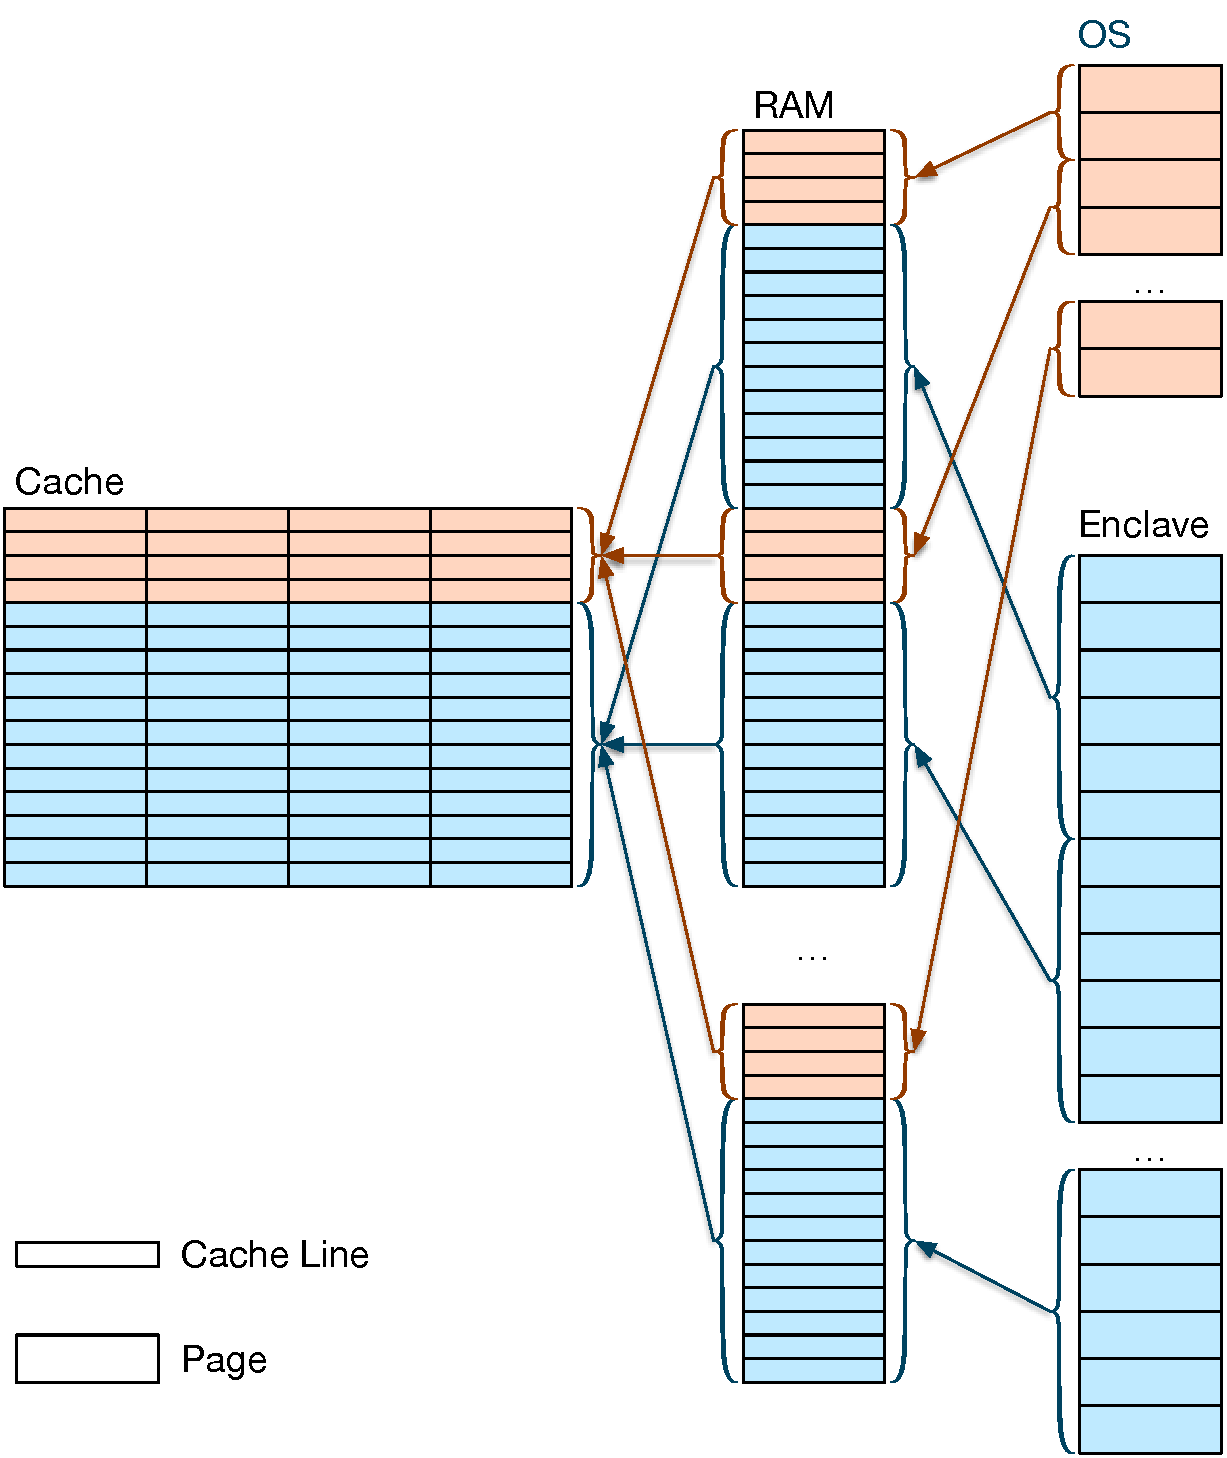
\includegraphics[width=85mm]{figures/cache_partitions.pdf}}
  \caption{
    Cache partitioning between two applications. Each application has some
    cache sets allocated to it, and only uses RAM regions that map to its cache
    sets. When partitioning the L1 cache, applications have to follow this
    constraint themselves. When the L2 cache is partitioned, the OS can map the
    pages in an application's virtual address space to the RAM regions that the
    application can use, so applications are oblivious to the cache
    partitioning.
  }
  \label{fig:cache_partitions}
\end{figure}

